\documentclass[twoside]{article}
\setlength{\oddsidemargin}{0 in}
\setlength{\evensidemargin}{0 in}
\setlength{\topmargin}{-0.6 in}
\setlength{\textwidth}{6.5 in}
\setlength{\textheight}{8.5 in}
\setlength{\headsep}{0.75 in}
\setlength{\parindent}{0 in}
\setlength{\parskip}{0.1 in}

\usepackage{url}
\usepackage{titlesec}
\setcounter{secnumdepth}{3}
\usepackage{palatino}
\usepackage{marginnote}
\usepackage{multirow}
\usepackage{easybmat,bigdelim,arydshln}
\usepackage[authoryear,round]{natbib}
\usepackage{amssymb,amsmath,amsthm,amsfonts}
\usepackage{mathtools}
%\usepackage{nicematrix}
\usepackage{arydshln}
\usepackage{caption}
\usepackage{hyperref}
\usepackage{tcolorbox}
\tcbuselibrary{skins, breakable, theorems}
\usepackage{newpxtext,newpxmath}
\usepackage{longtable}
\usepackage{enumitem}
\makeatletter

\let\bar\overline

\setlist[itemize]{topsep=0pt,leftmargin=10pt,itemsep=-0.2em}
\usepackage{xcolor}
\usepackage{tikz}
\usepackage{pgfplots}
\pgfplotsset{compat = newest}
\usetikzlibrary{patterns,decorations.pathreplacing,decorations.markings,fit,shapes.geometric,angles,quotes,arrows}
\usepgfplotslibrary{fillbetween}

\usepackage{ifthen}
\usepackage{tikz-3dplot}

\pgfdeclarelayer{ft}
\pgfdeclarelayer{bg}
\pgfsetlayers{bg,main,ft}

\hypersetup{
    colorlinks,
    citecolor=red,
    filecolor=black,
    linkcolor=violet,
    urlcolor=blue
}

\definecolor{myblue}{cmyk}{1,.72,0,.38}
\definecolor{mypurple}{cmyk}{.57,1,0,.58}
\definecolor{myred}{cmyk}{0,.88,.88,.58}
\definecolor{mygreen}{cmyk}{1,0,.69,.66}
\definecolor{myorange}{cmyk}{0,.58,100,.20}
\definecolor{glaucous}{rgb}{0.38, 0.51, 0.71}

\makeatletter
\renewcommand{\thefigure}{\thesection.\arabic{figure}}
\newtheoremstyle{indented}
  {3pt}% space before
  {3pt}% space after
  {\addtolength{\@totalleftmargin}{3.5em}
   \addtolength{\linewidth}{-3.5em}
   \parshape 1 3.5em \linewidth}% body font
  {}% indent
  {\bfseries}% header font
  {.}% punctuation
  {.5em}% after theorem header
  {}% header specification (empty for default)
\makeatother

\newcommand{\ind}{\perp\!\!\!\perp}

\theoremstyle{definition}
\newtheorem{defin}{Definition}[section] % Creates a new counter, number within section
\newtheorem{prt}[defin]{Remark} 
\newtheorem{prts}[defin]{Remarks} % Again share defin's counter
\newtheorem{exmp}[defin]{Example} % etc.
\newtheorem{exmps}[defin]{Examples}
\newtheorem*{note}{Note}
\tcbuselibrary{theorems}

% use counter*=defin to make each tcbtheorem share defin's counter

\newtcbtheorem[use counter*=defin, number within=section]{definition}{Definition}{enhanced, breakable,
    colback = white, colframe = red!55!black, colbacktitle = red!55!black, attach boxed title to top left = {yshift = -2.5mm, xshift = 3mm}, boxed title style = {sharp corners},fonttitle=\bfseries}{def}

\newtcbtheorem[use counter*=defin, number within=section]{theorem}{Theorem}{enhanced, breakable,
    colback = white, colframe = blue!45!black, colbacktitle = blue!45!black, attach boxed title to top left = {yshift = -2.5mm, xshift = 3mm}, boxed title style = {sharp corners},fonttitle=\bfseries}{thm}
    
\newtcbtheorem[use counter*=defin, number within=section]{proposition}{Proposition}{enhanced, breakable,
    colback = white, colframe = teal, colbacktitle = teal, attach boxed title to top left = {yshift = -2.5mm, xshift = 3mm}, boxed title style = {sharp corners},fonttitle=\bfseries}{prop}

\newtcbtheorem[use counter*=defin, number within=section]{lemma}{Lemma}{enhanced, breakable,
    colback = white, colframe = orange!80!black, colbacktitle = orange!80!black, attach boxed title to top left = {yshift = -2.5mm, xshift = 3mm}, boxed title style = {sharp corners},fonttitle=\bfseries}{lemma}

\newtcbtheorem[use counter*=defin, number within=section]{example}{Example}{enhanced, breakable,
    colback = white, colframe = yellow!60!black, colbacktitle = yellow!60!black, attach boxed title to top left = {yshift = -2.5mm, xshift = 3mm}, boxed title style = {sharp corners},fonttitle=\bfseries}{exmp}

\newtcbtheorem[use counter*=defin, number within=section]{assumption}{Assumption}{enhanced, breakable,
    colback = white, colframe = violet!60!white, colbacktitle = violet!60!white, attach boxed title to top left = {yshift = -2.5mm, xshift = 3mm}, boxed title style = {sharp corners},fonttitle=\bfseries}{assump}

\newtcbtheorem[use counter*=defin, number within=section]{algorithm}{Algorithm}{enhanced, breakable,
    colback = white, colframe = green!55!black, colbacktitle = green!55!black, attach boxed title to top left = {yshift = -2.5mm, xshift = 3mm}, boxed title style = {sharp corners},fonttitle=\bfseries}{algm}
%\newtcolorbox{example}[1]{enhanced, breakable, colback = white, colframe = orange!85!black, colbacktitle = orange!85!black, attach boxed title to top left = {yshift = -2.5mm, xshift = 3mm}, boxed title style = {sharp corners},fonttitle=\bfseries, title={Example: #1}}

\newtcbox{\myhl}[1][white]
  {on line, arc = 0pt, outer arc = 0pt,
    colback = #1!20!white, colframe = #1!50!black,
    boxsep = 0pt, left = 1pt, right = 1pt, top = 1pt, bottom = 1pt, boxrule = 0pt, bottomrule =0pt, toprule =0pt}
    
\newtcbox{\myhlrule}[1][white]
  {on line, arc = 0pt, outer arc = 0pt,
    colback = #1!20!white, colframe = #1!50!black,
    boxsep = 0pt, left = 1pt, right = 1pt, top = 1pt, bottom = 1pt, boxrule = 0pt, bottomrule =0.5pt, toprule =0.5pt}
%
% The following commands set up the lecnum (lecture number)
% counter and make various numbering schemes work relative
% to the lecture number.
%
\newcounter{lecnum}
\renewcommand{\thepage}{\thelecnum-\arabic{page}}
\renewcommand{\thesection}{\thelecnum.\arabic{section}}
\renewcommand{\theequation}{\thelecnum.\arabic{equation}}
\renewcommand{\thefigure}{\thelecnum.\arabic{figure}}
\renewcommand{\thetable}{\thelecnum.\arabic{table}}

\newcommand{\sidenotes}[1]{\marginnote{\raggedright\scriptsize#1}}
%
% The following macro is used to generate the header.
%
\newcommand{\lecture}[6]{
   \pagestyle{myheadings}
   \thispagestyle{plain}
   \newpage
   \setcounter{lecnum}{#1}
   \setcounter{page}{1}
   \noindent
   \begin{center}
   \framebox{
      \vbox{\vspace{2mm}
    \hbox to 6.28in { {\bf Econometrics
	\hfill \today} }
       \vspace{4mm}
       \hbox to 6.28in { {\Large \hfill Topic #1: #2  \hfill} }
       \vspace{2mm}
       \hbox to 6.28in { {\it #3 \hfill by #4} }
      \vspace{2mm}}
   }
   \end{center}
   \markboth{Week #1: #2}{Week #1: #2}

   {\bf Key points}: {#5}

   {\bf Disclaimer}: {\it #6}
   \vspace*{4mm}
}
%

\tikzset{-stealth-/.style={decoration={
  markings,
  mark=at position #1 with {\arrow{stealth}}},postaction={decorate}}}

  \tikzset{tangent/.style={
    decoration={
        markings,% switch on markings
        mark=
            at position #1
            with
            {
                \coordinate (tangent point-\pgfkeysvalueof{/pgf/decoration/mark info/sequence number}) at (0pt,0pt);
                \coordinate (tangent unit vector-\pgfkeysvalueof{/pgf/decoration/mark info/sequence number}) at (1,0pt);
                \coordinate (tangent orthogonal unit vector-\pgfkeysvalueof{/pgf/decoration/mark info/sequence number}) at (0pt,1);
            }
    },
    postaction=decorate
},
use tangent/.style={
    shift=(tangent point-#1),
    x=(tangent unit vector-#1),
    y=(tangent orthogonal unit vector-#1)
},
use tangent/.default=1}

\tikzstyle{terminator} = [rectangle, draw, thick, text centered, rounded corners, minimum height=2em]
\tikzstyle{process} = [rectangle, draw, thick, text centered, minimum height=2em]
\tikzstyle{decision} = [diamond, draw, thick, text centered, minimum width=3cm, minimum height=0.5cm]
\tikzstyle{data}=[trapezium, draw, thick, text centered, trapezium left angle=60, trapezium right angle=120, minimum height=2em]
\tikzstyle{arrow} = [thick,->,>=stealth]

\begin{document}
\lecture{18}{Eigenvalue and Spike Models}{}{Sai Zhang}{.}{The note is built on Prof. \hyperlink{http://faculty.marshall.usc.edu/jinchi-lv/}{Jinchi Lv}'s lectures of the course at USC, DSO 607, High-Dimensional Statistics and Big Data Problems.}
%\footnotetext{These notes are partially based on those of Nigel Mansell.}

\section{Motivation}
Consider $n$ independent observations $\mathbf{X}_i\in \mathbb{R}^p$ drawn from a $\mathcal{N}(\mathbf{0},\boldsymbol{\Sigma})$, then the covariance can be decomposed into 2 parts, white noise and low rank
\begin{align*}
    \boldsymbol{\Sigma} = \mathrm{Cov}(\mathbf{X}_i) = \mathbf{I} + \sum^M_{k=1}\theta_k \nu_k\nu'_k =\boldsymbol{\Sigma}_0 + \boldsymbol{\Phi}
\end{align*}
where $M$ denotes the \myhl[myblue]{\textbf{number of spikes}} in the distribution of eigenvalues. The idea is: spikes deviate from a reference model along a \textbf{\underline{small fixed number}} of unknown directions. If $\boldsymbol{\Phi}=\mathbf{0}$, then none of the sample eigenvalues is separated from the bulk.

\paragraph*{Why a spike model is interesting?} A spike model can help determine the latent dimension of the data, some examples being
\begin{itemize}
    \item Principal component analysis (PCA): spikes are related to the directions of the most variations of the data, i.e., the principal components
    \item Clustering model: $M$ spikes is equivalent to $M+1$ clusters
    \item Economic significance: $M$ is related to the number of factor loadings
\end{itemize}

Then the question is threefold: 
\begin{itemize}
    \item[-] How to determine $M$
    \item[-] How to estimate $\nu_k$
    \item[-] How to test $\theta_k$
\end{itemize}

Under rank one alternative, we would like to test the hypothesis
$$
H_1: \boldsymbol{\Sigma} = \mathbf{I}_p+ \theta\boldsymbol{\nu}\boldsymbol{\nu}', \theta>0
$$
against the null
\begin{align*}
    H_0 &: \boldsymbol{\Sigma}= \mathbf{I}_p
\end{align*}
with the key assumptions:
\begin{itemize}
    \item[A1] Gaussian error
    \item[A2] large $p$: $p\leq n$ but allows $p/n \rightarrow \gamma \in (0,1)$ 
\end{itemize}
Under these assumptions, for the $n\times p$ data matrix $\mathbf{X} = \begin{pmatrix}
    \mathbf{X}'_1 &\cdots & \mathbf{X}'_n
\end{pmatrix}'$, $\mathbf{X}'\mathbf{X}$ has a $p-$dimensional \myhl[myblue]{\textbf{Wishart} distribution $W_p(n,\boldsymbol{\Sigma})$} with the degree of freedom $n$ and covariance matrix $\boldsymbol{\Sigma}$, which is a \textit{random matrix}.

If $\mathbf{Y} = \mathbf{M} + \mathbf{X}$, that is, the sum of the \textit{random matrix} $\mathbf{X}$ and a \textit{deterministic matrix} $\mathbf{M}$ (also $n\times p$), then $\mathbf{Y}'\mathbf{Y}$ has a $p-$dimensional Wishart distribution $W_p(n,\boldsymbol{\Sigma},\boldsymbol{\Psi})$ with $n$ degrees of freedom, covariance matrix $\boldsymbol{\Sigma}$ and non-centrality matrix $\boldsymbol{\Psi}=\boldsymbol{\Sigma}^{-1}\mathbf{M}'\mathbf{M}$.
\begin{definition}{Density of Wishart Distribution}{wishart_pdf}
    The PDF of Wishart distribution is defined as 
    \begin{align*}
        f(\mathbf{X}) = \frac{1}{2^{np/2}{\Gamma}_p\left(\frac{n}{2}\right)\left\vert \boldsymbol{\Sigma}\right\vert^{n/2} } \left\vert \mathbf{X} \right\vert^{(n-p-1)/2}\exp \left(-\frac{1}{2}\mathrm{tr}\left(\boldsymbol{\Sigma}^{-1}\mathbf{X}\right)\right)
    \end{align*}
    where $\mathbf{X}$ is a symmetric positive semidefinite and ${\Gamma}_p\left(\frac{n}{2}\right)$ is a multivariate gamma function such that 
    \begin{align*}
        {\Gamma}_p\left( \frac{n}{2} \right) = \pi^{\frac{p(p-1)}{4}} \prod^p_{j=1}{\Gamma}\left(\frac{n}{2}-\frac{j-1}{2}\right)
    \end{align*}
    Notice that the sample covariance matrix $\mathbf{S}=\frac{1}{n}\mathbf{X}'\mathbf{X}$ is just a scaled version of Wishart distribution
    $$
        n\mathbf{S} = \mathbf{X}'\mathbf{X} \sim W_p(n,\boldsymbol{\Sigma})
    $$
\end{definition}
For $\boldsymbol{\Sigma}=\mathbf{I}_p$, the empirical distribution fo eigenvalues converges to Marcenko-Pastur distribution
\begin{align*}
    f^{\mathrm{MP}}(x) = \frac{1}{2\pi\gamma x}\sqrt{(b_+-x)(x-b_-)}
\end{align*}
where $b_{\pm} = (1\pm \sqrt{\gamma})^2$. Then:
\begin{itemize}
    \item under $H_0: \boldsymbol{\Sigma}= \mathbf{I}_p$, we have 
    $$
    n^{2/3}\left( \frac{\lambda_1 -\mu(\gamma)}{\sigma (\gamma)} \right) \xrightarrow{d} \mathrm{TW}_1
    $$
    where $\mathrm{TW}_1$ is the Tracy-Widom distribution
    \item under $H_1: \boldsymbol{\Sigma} = \mathbf{I}_p+ \theta\boldsymbol{\nu}\boldsymbol{\nu}', \theta>0$, if $\theta$ is strong ($\theta\gg \sqrt{\gamma}$), then
    $$
    n^{1/2}\left( \frac{\lambda_1 - \rho(\theta,\gamma)}{\tau (\theta,\gamma)} \right) \xrightarrow{d}\mathcal{N}(0,1)
    $$
\end{itemize}
Here, the largest eigenvalue test is the best test. \textbf{But} when the signal is weak $(0 \leq \theta < \sqrt{\gamma})$, the largest eigenvalue under the alternative converges to the same distribution as null: 
\begin{align*}
    n^{2/3} \left( \frac{\lambda_1 - \rho(\theta,\gamma)}{\tau (\theta,\gamma)} \right) \xrightarrow{d} \mathrm{TW}_1
\end{align*}
which means that the largest eigenvalue test \textit{fails}. On top of this, \textbf{resampling} also fails when $p$ is large.
\begin{figure}[ht]
    \centering
    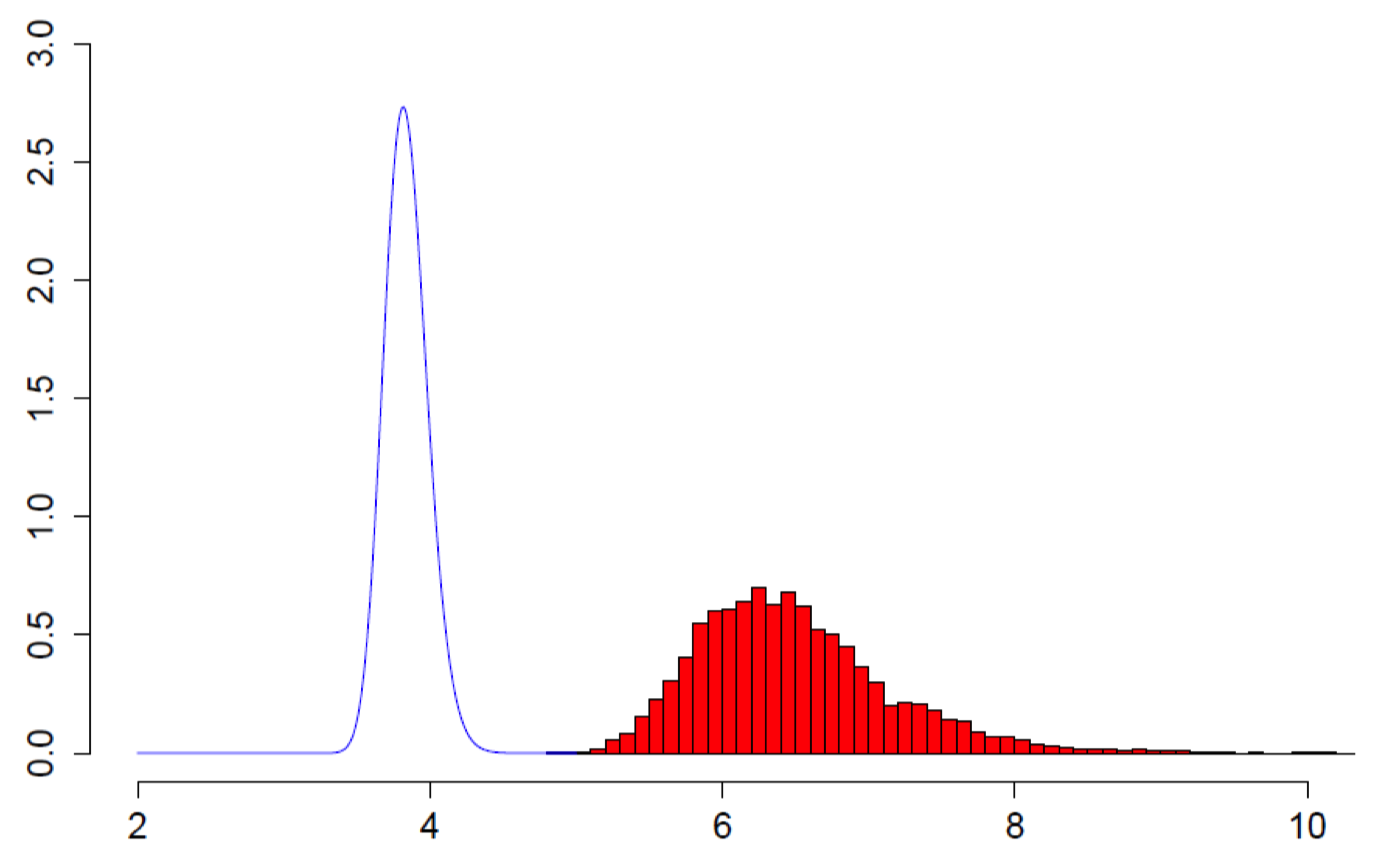
\includegraphics[width = 0.6 \textwidth]{figures/note18_resamplingfail.png}
    \caption{Failure of Resampling Test $(n=p=100)$}\label{fig:resampling_failure}
\end{figure}

Next, we develop another test to cope with these problems.

\section{Johnstone and Onatski (2020)}
Consider the basic equation of classical multivariate statistics:
\begin{align}\label{eq:multivariate_statistic}
    \det \left( \mathbf{H}-\mathbf{xE}\right) = 0
\end{align}
with $p\times p$ matrices
\begin{align*}
    n_1\mathbf{H} &= \sum^{n_1}_{k=1}\mathbf{x}_k\mathbf{x}_k' &\text{\textit{hypothesis} SS}\\
    n_1\mathbf{E} &= \sum^{n_1}_{k=1}\mathbf{z}_k\mathbf{z}_k' &\text{\textit{error} SS}
\end{align*}
The solution $\mathbf{x}$ is generalized eigenvalues $\left\{ \lambda_i \right\}^p_{i=1}$, which are the eigenvalue of \myhl[myblue]{F-ratio} $\mathbf{E}^{-1}\mathbf{H}$. \citet{johnstone2020testing} summarized 5 topics using $\mathbf{E}^{-1}\mathbf{H}$ relying on the five most common hypergeometric functions\footnote{Hypergeometric functions are:
\begin{itemize}
\item scalar inputs $$ _{\mathrm{p}}\mathcal{F}_{\mathrm{q}}(a,b;x) = \sum^{\infty}_{k=0} \frac{(a_1)_k\cdots (a_p)_k}{(b_1)_k\cdots (b_p)_k}\frac{x^k}{k!} $$ where $(a_j)_k$ are generalized Pochhammer symbols
\item single matrix inputs, where $\mathbf{S}$ is symmetric and usually diagonal $$ _{\mathrm{p}}\mathcal{F}_{\mathrm{q}}(a,b;\mathbf{S}) = \sum^{\infty}_{k=0} \sum_{\kappa} \frac{(a_1)_{\kappa}\cdots (a_p)_{\kappa}}{(b_1)_{\kappa}\cdots (b_p)_{\kappa}}\frac{C_{\kappa}(\mathbf{S})}{k!}  $$ where $C_k$ are the zonal polynomials. Easily, $ _{\mathrm{0}}\mathcal{F}_{\mathrm{0}}(\mathbf{S}) = e^{\mathrm{tr}(\mathbf{S})}$, $ _{\mathrm{1}}\mathcal{F}_{\mathrm{0}}(a,\mathbf{S}) = \left\vert \mathbf{I-S} \right\vert^{-a}$
\item two matrix inputs, where $\mathbf{S,T}$ are both symmetric $$ _{\mathrm{p}}\mathcal{F}_{\mathrm{q}}(a,b;\mathbf{S,T})  = \int_{O(p)} {}_{\mathrm{p}}\mathcal{F}_{\mathrm{q}} (a,b;\mathbf{SUTU'})\mathrm(d)\mathbf{U} $$
\end{itemize} } $_{\mathrm{p}}\mathcal{F}_{\mathrm{q}}$

\begin{table}[ht]
    \caption{5 Statistical Methods}\label{tab:5cases_James}
    \footnotesize
    \begin{center}
      \begin{tabular}{lccccc}
        
        \multicolumn{3}{c}{Statistical method} & $n_1\mathbf{H}$ & $n_2\mathbf{E}$ & Univariate Analog \\
        \hline
        $_{\mathrm{0}}\mathcal{F}_{\mathrm{0}}$ & PCA & Principal components analysis & $W_p(n_1,\boldsymbol{\Sigma+\Phi})$ & $n_2\boldsymbol{\Sigma}$ & $\chi^2$\\
        $_{\mathrm{1}}\mathcal{F}_{\mathrm{0}}$ & SigD & Signal detection & $W_p(n_1,\boldsymbol{\Sigma+\Phi})$ & $W_p(n_2,\boldsymbol{\Sigma})$ & non-central $\chi^2$ \\
        $_{\mathrm{0}}\mathcal{F}_{\mathrm{1}}$ & REG$_0$ & Multivariate regression, with known error & $W_p(n_1,\boldsymbol{\Sigma},n_1\boldsymbol{\Phi})$ & $n_2\boldsymbol{\Sigma}$ & $F$ \\
        $_{\mathrm{1}}\mathcal{F}_{\mathrm{1}}$ & REG & Multivariate regression, with unknown error & $W_p(n_1,\boldsymbol{\Sigma},n_1\boldsymbol{\Phi})$ & $W_p(n_2,\boldsymbol{\Sigma})$ & non-central $F$ \\
        $_{\mathrm{2}}\mathcal{F}_{\mathrm{1}}$ & CCA & Canonical correlation analysis & $W_p(n_1,\boldsymbol{\Sigma},\boldsymbol{\Phi}(\mathbf{Y}))$ & $W_p(n_2,\boldsymbol{\Sigma})$ & $\frac{r^2}{1-r^2}$\\ \hline
        \multicolumn{5}{l}{For $_{\mathrm{0}}\mathcal{F}_{\mathrm{0}}$ and $_{\mathrm{0}}\mathcal{F}_{\mathrm{1}}$, $\mathbf{E}$ is deterministic, $\boldsymbol{\Sigma}$ is known, $n_2$ disppears, otherwise $\mathbf{E}$ is independent of $\mathbf{H}$.}
      \end{tabular}
    \end{center}
\end{table}

\subsection{Definitions and global assumptions}
Let $\mathbf{Z}$ be an $n\times p$ data matrix with rows (observations) drawn \textbf{i.i.d.} from $\mathcal{N}_p(\mathbf{0},\boldsymbol{\Sigma})$, and a deterministic matrix $\mathbf{M}$ of $n\times p$, then for $\mathbf{Y} = \mathbf{M}+ \mathbf{Z}$, 
\begin{itemize}
    \item $\mathbf{H} = \mathbf{Y'Y}$ has a $p$ dimensional Wishart distribution $W_p(n,\boldsymbol{\Sigma,\Psi})$ with $n$ degrees of freedom, covariance matrix $\boldsymbol{\Sigma}$ and non-centrality matrix $\boldsymbol{\Psi}=\boldsymbol{\Sigma}^{-1}\mathbf{M'M}$
    \item the corresponding central Wishart distribution with $\mathbf{M}=\mathbf{0}$ is $W_p(n,\boldsymbol{\Sigma})$
\end{itemize}
\citet{johnstone2020testing} assume a relative low dimensionality $p\leq \min\left\{ n_1,n_2 \right\}$ where $n_1,n_2$ are the degrees of freedom as in Table \ref{tab:5cases_James}, where 
\begin{itemize}
    \item[-] $p\leq n_2$ ensures almost sure invertibility of matrix $\mathbf{E}$ in Equation \ref{eq:multivariate_statistic} 
    \item[-] $p\leq n_1$ is not essential, but reduces the number of various situations of consideration.
\end{itemize}

\subsection{5 classes of problems}
With these assumptions, they established a unified statistical problem \myhl[myblue]{\textbf{symmetric matrix denoising (SMD)}} that can be linked to the 5 classes of problems:

\paragraph*{PCA} $n_1$ i.i.d. observations drawn from $\mathcal{N}_p(\mathbf{0},\boldsymbol{\Omega})$ to test the hull hypothesis that the population covariance $\boldsymbol{\Omega} = \boldsymbol{\Sigma}$, with the alternative of interest being $$ \boldsymbol{\Omega} = \boldsymbol{\Sigma+\Phi},\ \text{ with }\boldsymbol{\Phi}=\theta \boldsymbol{\phi\phi'}  $$ where $\theta>0$, $\boldsymbol{\phi}$ are unknown, and $\boldsymbol{\phi}$ is normalized s.t. $\left\Vert \boldsymbol{\Sigma}^{-1/2}\boldsymbol{\phi} \right\Vert = 1$. W.L.O.G., assume $\boldsymbol{\Sigma}=\mathbf{I}_p$, then under the alternative, the first principal component explains a larger portion of the variation than the other principal components. Re-formulate the hypotheses in terms of the spectral \textit{spike} parameter $\theta$, we have
\begin{align}\label{eq:spectral_spike_hypotheses}
    H_0: \theta_0 &= 0 & H_1: \theta_0 = \theta>0
\end{align}
where $\theta_0$ is the true value of the \textit{spike}. A \myhl[myblue]{\textbf{maximal invariant statistic}} consists of the solutions $\lambda_1\geq \cdots\geq \lambda_p$ of Equation \ref{eq:multivariate_statistic} with
\begin{itemize}
    \item $n_1\mathbf{H}$ equal to the sample covariance matrix
    \item $\mathbf{E} = \boldsymbol{\Sigma}$
\end{itemize}

\paragraph*{SigD} Now consider testing the \textbf{equality} of covariance matrices $\boldsymbol{\Omega}$ and $\boldsymbol{\Sigma}$, corresponding to 2 independent $p-$dimensional mean-zero Gaussian samples of size \myhl[myblue]{$n_1$} and \myhl[myblue]{$n_2$}, with the alternative still  $$ \boldsymbol{\Omega} = \boldsymbol{\Sigma+\Phi},\ \text{ with }\boldsymbol{\Phi}=\theta \boldsymbol{\phi\phi'}  $$ and again, assume $\boldsymbol{\Sigma}=\mathbf{I}_p$ (but NOT necessarily known), here, instead of Equation \ref{eq:multivariate_statistic}, consider 
\begin{align}
    \det \left( \mathbf{H}-\boldsymbol{\lambda}\left(\mathbf{E}+\frac{n_1}{n_2}\mathbf{H}\right) \right) = 0
\end{align}
naturally, SigD reduces to PCA as $n_2\rightarrow\infty$ while $n_1$ and $p$ held constant.

\paragraph*{REG$_0$} Next, consider a linear regression with multivariate response $$ \mathbf{Y} = \mathbf{X}\boldsymbol{\beta} + \boldsymbol{\epsilon} $$ with known covariance matrix $\boldsymbol{\Sigma}$ of the i.i.d. Gaussian rows of the error matrix $\boldsymbol{\epsilon}$. Here, to test linear restrictions on the matrix of coefficients $\boldsymbol{\beta}$, we can split the matrix of transformed response variables $\mathbf{Y}$ into 3 parts $\mathbf{Y}_1,\mathbf{Y}_2,\mathbf{Y}_3$, where 
\begin{itemize}
    \item $\mathbf{Y}_1$ is $n_1\times p$ where $p$ is the number of response variables, $n_1$ is the number of linear restrictions (per each of the $p$ columns of matrix $\boldsymbol{\beta}$), under the null $H_0: \mathbb{E}\mathbf{Y}_1 = 0$, versus the alternative \begin{align}\label{eq:REG_alternative}
        \mathbb{E}\mathbf{Y}_1 = \sqrt{n_1\theta}\boldsymbol{\psi\phi'}
    \end{align}
    where $\theta>0$, $\left\Vert \boldsymbol{\Sigma}^{-1/2}\boldsymbol{\phi}\right\Vert = 1$ and $\lVert \boldsymbol{\psi}\rVert = 1$
    \item $\mathbf{Y}_2$ is $(q-n_1)\times p$, where $q$ is the number of regressors
    \item $\mathbf{Y}_3$ is $(T-q)\times p$, where $T$ is the number of observations
\end{itemize}
In this case, tests can be based on the solutions $\lambda_1,\cdots,\lambda_p$ to $$ \det \left( \mathbf{H}-\boldsymbol{\lambda }\mathbf{E} \right)=\mathbf{0} $$
where $\mathbf{H} = \mathbf{Y}'_1\mathbf{Y}_1/n_1$ and $\mathbf{E}=\boldsymbol{\Sigma}$. The solutions represent a multivaraite analog of the difference between the sum of squared residuals in the restircted and unrestricted regressions. Under the null, $n_1\mathbf{H}$ is distributed as $W_p(n_1,\boldsymbol{\Sigma})$. Here, 
\begin{align*}
    n_1\mathbf{H} & \sim W_p(n_1,\boldsymbol{\Sigma}) & \text{under }H_0\\
    n_1\mathbf{H} & \sim W_p(n_1,\boldsymbol{\Sigma},n_1\boldsymbol{\Phi}),\ \text{where }\boldsymbol{\Phi} = \theta \boldsymbol{\Sigma}^{-1}\boldsymbol{\phi\phi}' & \text{under }H_1
\end{align*}
Again, W.L.O.G, assume $\boldsymbol{\Sigma} = \mathbf{I}_p$. This \myhl[myblue]{\textbf{canonical form}} of REG$_0$ is essentially equivalent to the setting of \textbf{\underline{matrix denoising}}
$$
\mathbf{Y}_1 = \mathbf{M}+ \mathbf{Z}
$$

\paragraph*{REG} Again, consider the linear regression $$ \mathbf{Y} = \mathbf{X}\boldsymbol{\beta} + \boldsymbol{\epsilon} $$ but \textbf{NOT} knowing the covariance matrix $\boldsymbol{\Sigma}$ of rows of $\boldsymbol{\epsilon}$. Here, the solutions again solve $\det \left( \mathbf{H}-\boldsymbol{\lambda }\mathbf{E} \right)=\mathbf{0}$ with $$ \mathbf{H} = \mathbf{Y}'_1\mathbf{Y}_1/n_1,\ \mathbf{E}=\mathbf{Y}'_3\mathbf{Y}_3/n_2 $$
this represents a multivariate analog of the $F$ ratio: the difference between the sum of squared residuals in the restricted and unrestricted regressions to the sum of squared residuals in the restricted regression. Again, as $n_2 \rightarrow \infty$, REG reduces to REG$_0$. 

\paragraph*{CCA} Consider testing for independence between Gaussian vectors $x_t\in\mathbb{R}^p$ and $y_t\in \mathbb{R}^{n_1}$, given zero-mean observations with $t=1,\cdots,n_1+n_2$. Partition the population and sample covariance matrices of the observations $(x_t',y_t')'$ into 
\begin{align*}
    \begin{pmatrix}
        \boldsymbol{\Sigma}_{xx} & \boldsymbol{\Sigma}_{xy}\\
        \boldsymbol{\Sigma}_{yx} & \boldsymbol{\Sigma}_{yy}
    \end{pmatrix} & & \begin{pmatrix}
        \mathbf{S}_{xx} & \mathbf{S}_{xy}\\
        \mathbf{S}_{yx} & \mathbf{S}_{yy}
    \end{pmatrix}
\end{align*}
respsectively. Under $H_0:\boldsymbol{\Sigma}_{xy}=\mathbf{0}$, while the alternative is
\begin{align}
    \boldsymbol{\Sigma}_{xy} = \sqrt{\frac{n_1\theta}{n_1\theta + n_1 + n_2}}\boldsymbol{\phi\psi}'
\end{align}
where the nuisance parameters $\phi \in \mathbb{R}^p$ and $\psi \in \mathbb{R}^{n_1}$ are normalized s.t.
\begin{align*}
    \left\Vert \boldsymbol{\Sigma}_{xx}^{-1/2}\boldsymbol{\phi} \right\Vert = \left\Vert \boldsymbol{\Sigma}_{yy}^{-1/2}\boldsymbol{\psi} \right\Vert = 1
\end{align*}
And the test can be based on the squared sample canonical correlations $\lambda_1,\cdots,\lambda_p$ that solves $$ \det \left( \mathbf{H}-\boldsymbol{\lambda }\mathbf{E} \right)=\mathbf{0} $$
with
\begin{align*}
    \mathbf{H} &= \mathbf{S}_{xy}\mathbf{S}_{yy}^{-1}\mathbf{S}_{yx} & \mathbf{E}&\mathbf{S}_{xx}
\end{align*}

\subsection{SMD}
For a $\mathbf{X} = \boldsymbol{\Phi} + \mathbf{Z}/\sqrt{p}$ where $\mathbf{Z}$ is a noise matrix from the \myhl[myblue]{\textbf{Gaussian Orthogonal Ensemble} (GOE)}\footnote{$\mathbf{Z}$ is from the GOE that it is \textbf{symmetric} and \begin{align*} \mathbf{Z}_{ii} &\sim \mathcal{N}(0,2) & \mathbf{Z}_{ij}\sim\mathcal{N}(0,1) \text{ if }i>j \end{align*} }
We seek to make inference about a symmetric rank-one \textit{signal} matrix $\boldsymbol{\Phi} = \theta\boldsymbol{\phi\phi}'$. The null and the alternative is again as in \ref{eq:spectral_spike_hypotheses}. The nuisance vector $\boldsymbol{\phi}\in\mathbb{R}^p$ is normalized s.t. $\left\Vert \boldsymbol{\phi} \right\Vert =1$. 

The problem remains \myhl[myblue]{\textbf{invariant}} under the multiplication of $\mathbf{X}$ from the left by an orthogonal matrix, and from the right by its transpose.
A maximal invariant statistic consists of the solutions $\lambda_1,\cdots,\lambda_p$ to $\det \left( \mathbf{H}-\boldsymbol{\lambda }\mathbf{E} \right)=\mathbf{0} $ with $\mathbf{H}=\mathbf{X}$ and $\mathbf{E}=\mathbf{I}_p$.

SMD can be viewed as a degenerate version of the 5 classes of problems, as shown in Figure \ref{fig:smd_5classesofproblems}:
\begin{itemize}
    \item \myhl[myblue]{\textbf{SMD}}, \myhl[myblue]{\textbf{PCA}}, \myhl[myblue]{\textbf{REG$_0$}}: random $\mathbf{H}$ and deterministic $\mathbf{E}$
    \item \myhl[myblue]{\textbf{PCA}} and \myhl[myblue]{\textbf{SigD}} are \textit{parallel} to \myhl[myblue]{\textbf{REG$_0$}}
    \item \myhl[myblue]{\textbf{CCA}} has a different structure of $\mathbf{H}$ and $\mathbf{E}$
\end{itemize}

\begin{figure}[ht]
    \caption{SMD and 5 Classes of Statistical Problems}\label{fig:smd_5classesofproblems}
    \centering
      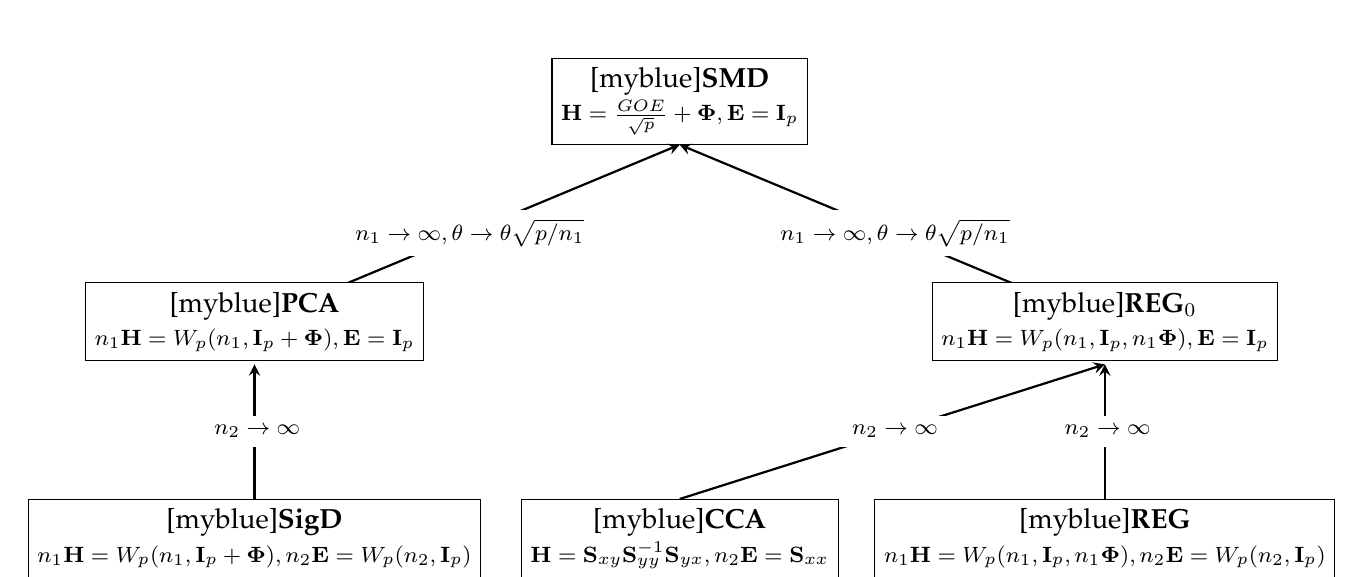
\begin{tikzpicture}[scale=0.9]
        \node[draw, above, align=center,fill=white] at (6,5) {\myhl[myblue]{\textbf{SMD}} \\ \footnotesize{$\mathbf{H}=\frac{GOE}{\sqrt{p}}+\boldsymbol{\Phi},\mathbf{E}=\mathbf{I}_p$}};
        
        \draw [-stealth,color=black,thick] (0,2.5) -- (6,5) node[midway, fill=white] {\footnotesize{ $n_1\rightarrow\infty,\theta\rightarrow\theta\sqrt{p/n_1}$ }};
        \node[draw, align=center,fill=white] at (0,2.5) {\myhl[myblue]{\textbf{PCA}} \\ \footnotesize{$n_1\mathbf{H}=W_p(n_1,\mathbf{I}_p+\boldsymbol{\Phi}),\mathbf{E}=\mathbf{I}_p$}};

        \draw [-stealth,color=black,thick] (12,2.5) -- (6,5) node[midway, fill=white] {\footnotesize{ $n_1\rightarrow\infty,\theta\rightarrow\theta\sqrt{p/n_1}$ }};
        \node[draw, align=center,fill=white] at (12,2.5) {\myhl[myblue]{\textbf{REG$_0$}} \\ \footnotesize{$n_1\mathbf{H}=W_p(n_1,\mathbf{I}_p,n_1\boldsymbol{\Phi}),\mathbf{E}=\mathbf{I}_p$}};

        \draw [-stealth,color=black,thick] (0,0) -- (0,1.9) node[midway, fill=white] {\footnotesize{ $n_2\rightarrow\infty$ }};
        \node[draw, below, align=center,fill=white] at (0,0) {\myhl[myblue]{\textbf{SigD}} \\ \footnotesize{$n_1\mathbf{H}=W_p(n_1,\mathbf{I}_p+\boldsymbol{\Phi}),n_2\mathbf{E}=W_p(n_2,\mathbf{I}_p)$}};

        \draw [-stealth,color=black,thick] (12,0) -- (12,1.9) node[midway, fill=white] {\footnotesize{ $n_2\rightarrow\infty$ }};
        \node[draw, below, align=center,fill=white] at (12,0) {\myhl[myblue]{\textbf{REG}} \\ \footnotesize{$n_1\mathbf{H}=W_p(n_1,\mathbf{I}_p,n_1\boldsymbol{\Phi}),n_2\mathbf{E}=W_p(n_2,\mathbf{I}_p)$}};

        \draw [-stealth,color=black,thick] (6,0) -- (12,1.9) node[midway, fill=white] {\footnotesize{ $n_2\rightarrow\infty$ }};
        \node[draw, below, align=center,fill=white] at (6,0) {\myhl[myblue]{\textbf{CCA}} \\ \footnotesize{$\mathbf{H}=\mathbf{S}_{xy}\mathbf{S}_{yy}^{-1}\mathbf{S}_{yx},n_2\mathbf{E}=\mathbf{S}_{xx}$}};
      \end{tikzpicture}
\end{figure}

\subsection{The likelihood ratios} The goal is to study the asymptotic behavior of likelihood ratios based on the observed eigenvalues 
$$
\Lambda = \mathrm{diag}\left\{ \lambda_1,\cdots,\lambda_p \right\}
$$
then the likelihood of the alternative versus the null is given by 
\begin{equation}\label{eq:likelihood_ratio}
    \mathcal{L}(\theta,\Lambda) = \frac{p(\Lambda;\theta)}{p(\Lambda;0)} = \alpha(\theta) _{\mathrm{p}}\mathcal{D}_{\mathrm{q}}(\mathbf{a,b};\boldsymbol{\Phi},\Lambda)
\end{equation}
where $\boldsymbol{\Phi}=\boldsymbol{\Phi}(\theta)$ is a $p$-dimensional matrix $\mathrm{diag}\left\{ \boldsymbol{\Phi}_{11},0,\cdots,0 \right\}$. Consider the hypergeometric functions of 2 matrix arguments $\boldsymbol{\Phi,\Lambda}$ are defined as 
\begin{align*}
    _{\mathrm{p}}\mathcal{F}_{\mathrm{q}}(\mathbf{a,b};\boldsymbol{\Phi,\Lambda}) &= \sum^{\infty}_{k=0} \frac{1}{k!}\sum_{\kappa-k}\frac{\left(a_1\right)_{\kappa}\cdots\left(a_{\mathrm{p}}\right)_{\kappa}}{\left(b_1\right)_{\kappa}\cdots\left(b_{\mathrm{1}}\right)_{\kappa}}\frac{C_{\kappa}(\boldsymbol{\Phi})C_{\kappa}(\boldsymbol{\Lambda})}{C_{\kappa}(\mathbf{I}_p)}
\end{align*}
where $\mathbf{a}=\left( a_1,\cdots,a_{\mathrm{p}} \right)$ and $\mathbf{b}=\left( b_1,\cdots,b_{\mathrm{q}} \right)$ are parameters, $\kappa$ are partitions of the integer $k$, $(a_j)_{\kappa}$ and $(b_i)_{\kappa}$ are the generalized Pochhammer symbols, $C_{\kappa}$ are the zonal polynomials. For each of the 6 classes of problems, we have the parameters as in Table  where $n = n_1+n_2 $.

\begin{table}[ht]
    \caption{Parameters of the Likelihood Ratios in Eq.\ref{eq:likelihood_ratio}}\label{tab:6cases_parameters}
    \footnotesize
    \begin{center}
      \begin{tabular}{lccccc}
        Classes & $_{\mathrm{p}}\mathcal{F}_{\mathrm{q}}$ & $\alpha(\theta)$ & $a$ & $b$ & $\boldsymbol{\Phi}_{11}$ \\
        \hline
        SMD & $_{\mathrm{0}}\mathcal{F}_{\mathrm{0}}$ & $\exp(-p\theta^2/4)$ & - & - & $\theta p/2$\\
        PCA & $_{\mathrm{0}}\mathcal{F}_{\mathrm{0}}$ & $(1+\theta)^{-n_1/2}$ & - & - & $\theta n_1/(2(1+\theta))$\\
        SigD & $_{\mathrm{1}}\mathcal{F}_{\mathrm{0}}$ & $(1+\theta)^{-n_1/2}$ & - & - & $\theta n_1/(n_2(1+\theta))$ \\
        REG$_0$ & $_{\mathrm{0}}\mathcal{F}_{\mathrm{1}}$ & $\exp(-n_1\theta/2)$ & - & $n_1/2$ & $\theta n_1^2/4$ \\
        REG & $_{\mathrm{1}}\mathcal{F}_{\mathrm{1}}$ & $\exp(-n_1\theta/2)$ & $n/2$ & $n_1/2$ & $\theta n_1^2/(2n_2)$ \\
        CCA & $_{\mathrm{2}}\mathcal{F}_{\mathrm{1}}$ & $(1+n_1\theta/n)^{-n/2} $ & $(n/2,n/2)$ & $n_1/2$ & $\theta n_1^2/(n_2^2 + n_2n_1(1+\theta))$
      \end{tabular}
    \end{center}
\end{table}

Some links in Fig.\ref{fig:smd_5classesofproblems} can also be established via asymptotic relations between hypergeometric functions. 

\paragraph*{Asymptotic behavior of the likelihood ratios} consider that as $n_1,n_2,p$ go to infinity so that
\begin{align}
    c_1 \equiv \frac{p}{n_1} &\rightarrow \gamma_1\in (0,1) & c_2 \equiv \frac{p}{n_2} & \rightarrow \gamma_2\in (0,1]
\end{align}

\newpage
\bibliographystyle{plainnat}
\bibliography{ref.bib}

\end{document}